\documentclass[12pt,a4paper]{article}

\usepackage[utf8]{inputenc}
\usepackage[T1]{fontenc}
\usepackage[brazilian]{babel}
\usepackage{geometry}

% Fonte semelhante ao template SBC
\usepackage{newtxtext}
\usepackage{newtxmath}

% Configuração do título
\usepackage{titling}

% Configuração das seções
\usepackage{titlesec}

\usepackage{changepage}

% Adiciona cor no texto
\usepackage{xcolor}

% Tabelas e links
\usepackage{array}
\usepackage{tabularx}
\usepackage{xurl}
\usepackage[colorlinks=true,urlcolor=blue,linkcolor=black]{hyperref}

% Parágrafo padrão
\newcommand{\paragrafo}[1]{%
    \begin{adjustwidth}{1cm}{1cm}
        \indent\indent #1
    \end{adjustwidth}
}

% Importação de Imagens
\usepackage{graphicx}

%image
\usepackage{float}

% Margens
\geometry{a4paper, top=1cm,
    bottom=2cm,
    left=1.5cm,
    right=1.5cm
}

% --------------------------------------------------
% Configurações globais
% --------------------------------------------------

% Título
\setlength{\droptitle}{-4em}
\pretitle{\begin{center}\Large\bfseries}
\posttitle{\end{center}}

% Seções
\titleformat{\section}
    {\normalfont\large\bfseries}
    {\thesection}
    {0.5em}
    {}

% Subseções
\titleformat{\subsection}
    {\normalfont\normalsize\bfseries}
    {\thesubsection}
    {1em}
    {}

\titlespacing*{\section}
    {0cm}  % recuo à esquerda
    {0.8em}  % espaço antes da section
    {0.3em}  % espaço depois da section

\titlespacing*{\subsection}
    {0.6cm}  % recuo à esquerda
    {0.5em}    % espaço antes
    {0.5em}  % espaço depois

% --------------------------------------------------
% Informações do documento
% --------------------------------------------------

\title{Dashboard de Enchentes em Porto Alegre: Simulação do INCT e Rotas na Enchente}

\author{
    \small\bfseries
    Lorenzo Ali$^{1}$,
    Sophia Mendes da Silveira$^{2}$
    \\[0.3em]
    \small\normalfont
    Pontifícia Universidade Católica do Rio Grande do Sul --
    Porto Alegre -- RS -- Brazil
    \\[0.1em]
    \footnotesize\ttfamily
    lorenzo.goncalves@edu.pucrs.br$^{1}$,
    sophia.mendes@edu.pucrs.br$^{2}$
}

\date{\small 25 de Novembro de 2026}

% --------------------------------------------------
% Documento
% --------------------------------------------------

\begin{document}

\maketitle

\section{Objetivo e visão geral}
    \paragrafo{Em maio de 2024, o Guaíba chegou a 5,35 m em Porto Alegre, a maior marca da história. Este dashboard procura responder, de forma rápida, a duas perguntas sobre cenários como esse: se o rio chegar a X metros, quais bairros e quantas pessoas são afetados? E o que outras bases de dados sobre enchentes acrescentam a essa resposta?}
    \begin{itemize}
        \item \textbf{Tela 1, Simulação do INCT:} mostra quantas pessoas, prédios e bairros são afetados em cada nível do Guaíba, de 3,0 m a 10,0 m, a partir da simulação do INCT SiMAI depois de limpa.
        \item \textbf{Tela 2, Rotas na enchente:} usa as manchas de inundação e as ruas da cidade para mostrar quais ruas ficam debaixo d'água em cada nível, como sair de uma área alagada e como ir de um ponto a outro sem passar pela água.
        \item \textbf{Tecnologia:} Python e Streamlit. O \textit{app.py} prepara os dados (coleta e limpeza de cada base, só quando o arquivo de saída ainda não existe) e abre as duas telas. A Tela 1 usa pandas e Plotly. A Tela 2 usa GeoPandas, NetworkX e PyDeck.
    \end{itemize}

\section{Dados e fontes}
    \paragrafo{O dashboard usa três bases. A coleta e a limpeza de cada uma estão no repositório e rodam pelo \textit{app.py}. O detalhe da limpeza do INCT está no relatório de limpeza de dados.}
    \begin{adjustwidth}{1cm}{1cm}
    \small
    \begin{tabularx}{\linewidth}{|>{\raggedright\arraybackslash}p{3.1cm}|>{\raggedright\arraybackslash}p{4.4cm}|X|}
        \hline
        \textbf{Base} & \textbf{Fonte} & \textbf{Obtenção e uso} \\ \hline
        Simulação do INCT SiMAI & Arquivo \textit{data.json} fornecido à turma. Prédios: OpenStreetMap. População: Censo IBGE 2022. & Entregue pelo INCT, em JSON. Alimenta a Tela 1. \\ \hline
        Cotas de inundação (3,00 m a 5,35 m) & Prefeitura de Porto Alegre (SMAMUS), serviço ArcGIS REST. & API, em GeoJSON, coletada em 25/11/2026. Alimenta as manchas da Tela 2. \\ \hline
        Eixos de logradouros & Prefeitura de Porto Alegre (SMAMUS), página Mapas Digitais. & Download automatizado do \textit{shapefile}, coletado em 25/11/2026. Alimenta as ruas da Tela 2. \\ \hline
    \end{tabularx}
    \end{adjustwidth}
    \vspace{0.5em}
    \begin{itemize}
        \item \textbf{INCT:} 6.674 linhas (94 bairros em 71 níveis). Corrigimos 24 valores de prédios afetados (zeros no meio da série e valores que diminuíam quando o rio subia).
        \item \textbf{Cotas:} os polígonos da fonte têm anéis inválidos pelo padrão OGC, então as geometrias foram reparadas, e os 25 níveis ficaram válidos. As coordenadas foram convertidas para SIRGAS 2000 / UTM 22S, para medir em metros.
        \item \textbf{Logradouros:} 31.416 segmentos, classificados em ruas (30.494), contornos de área (786), itens que não são ruas (98) e vias de pedestres (15). As rotas usam ruas e vias de pedestres.
    \end{itemize}

\section{Tela 1: Simulação do INCT}
    \subsection{Objetivo e como usar}
        \paragrafo{A tela responde: se o rio chegar a X metros, quais bairros e quantas pessoas são afetados? Um controle deslizante escolhe o nível do Guaíba, de 3,0 m a 10,0 m em passos de 0,1 m, e todos os elementos da tela se atualizam juntos.}
    \subsection{Visualizações e por que as escolhemos}
        \begin{itemize}
            \item \textbf{Indicadores no topo:} pessoas afetadas, prédios afetados, bairros atingidos (``x de 94'') e a parcela da população da cidade. Dão a resposta em números, sem precisar ler gráfico.
            \item \textbf{Curva da população afetada:} mostra como o impacto cresce conforme o rio sobe. Um ponto marca o nível escolhido, e uma linha tracejada marca o recorde de maio de 2024 (5,35 m), para dar uma referência conhecida.
            \item \textbf{Tabela dos bairros com mais pessoas afetadas:} os dez primeiros, com uma barra da porcentagem de prédios afetados. Separa ``quantas pessoas'' de ``quanto do bairro'', porque um bairro grande pode ter muita gente afetada e ainda assim uma parte pequena dos prédios.
            \item \textbf{Ranking de barras da porcentagem de prédios afetados:} compara todos os bairros atingidos em proporção, sem favorecer os maiores.
            \item \textbf{Fonte e limitações no rodapé:} deixam claro que os números são estimativas de uma simulação.
        \end{itemize}
        \paragrafo{Com o controle em 3,5 m, a simulação indica 58.066 pessoas afetadas, 22.443 prédios e 32 dos 94 bairros atingidos, o que equivale a 4,4\% da população. Farrapos aparece à frente, com 17.416 pessoas e 99\% dos prédios.}
        \begin{figure}[H]
            \centering
            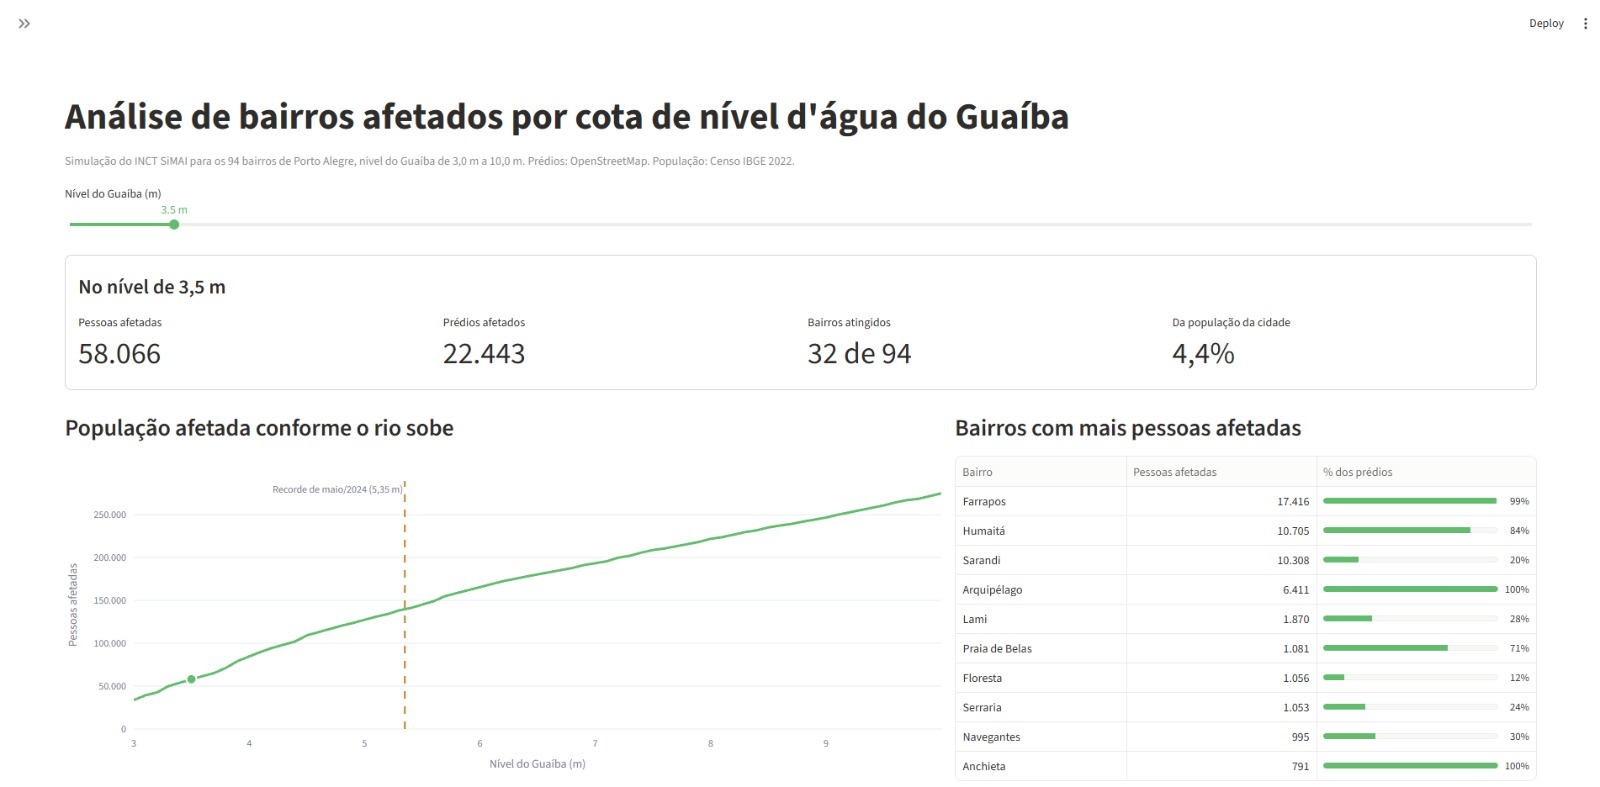
\includegraphics[width=0.9\textwidth]{assets/tela1_nivel_3_5.png}
            \caption{Tela 1 com o nível do Guaíba em 3,5 m.}
            \label{fig:tela1_35}
        \end{figure}
        \paragrafo{Movendo o controle para 7,7 m, os números sobem para 213.155 pessoas afetadas (16,0\% da população), 80.336 prédios e 48 bairros. Sarandi passa a liderar, com 36.078 pessoas e 70\% dos prédios. Na curva, a 5,3 m o arquivo limpo soma 138.414 pessoas afetadas.}
        \begin{figure}[H]
            \centering
            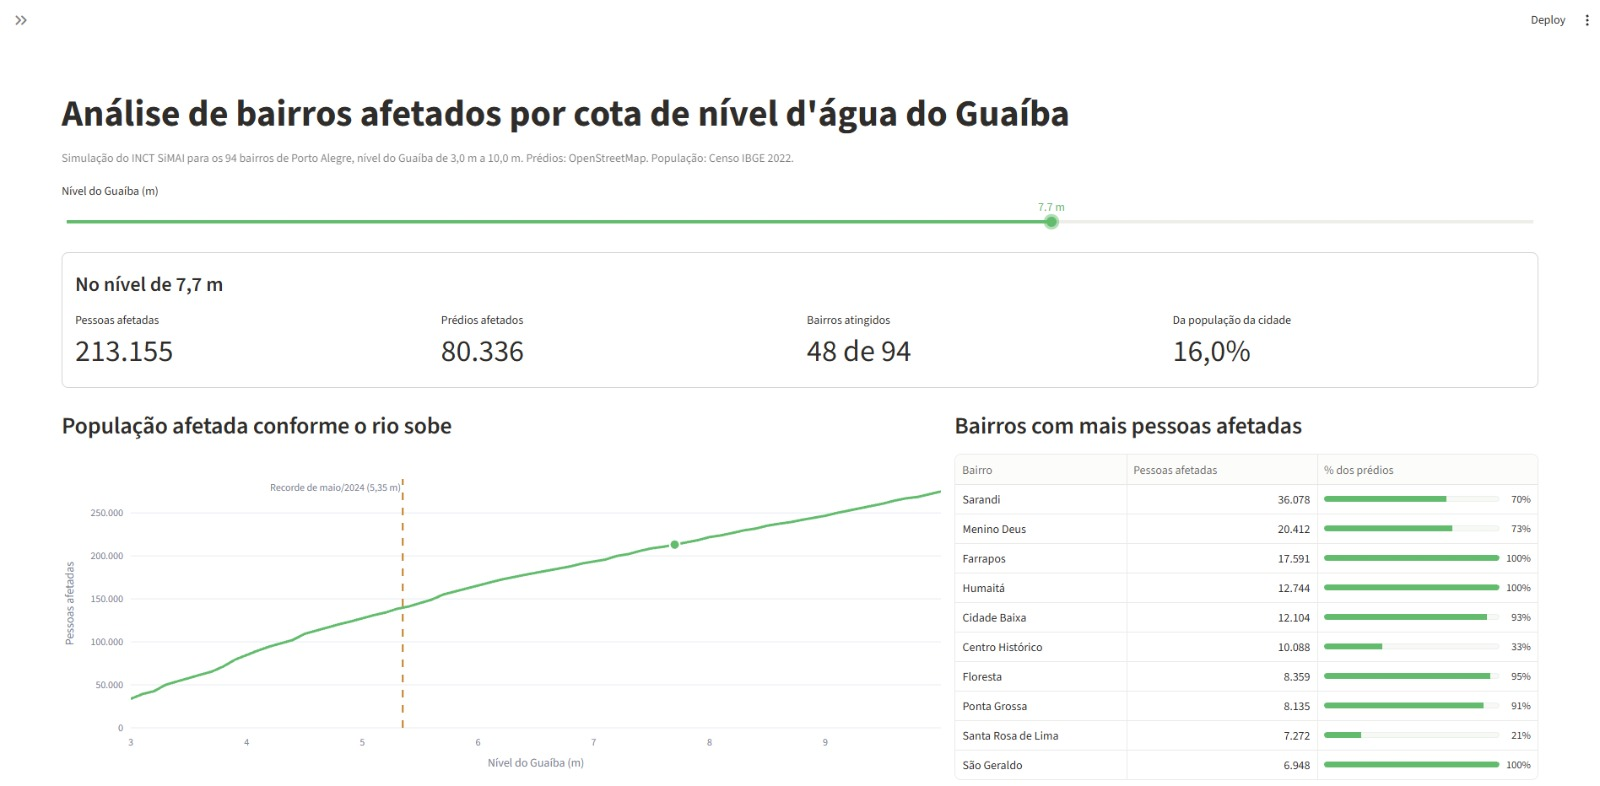
\includegraphics[width=0.9\textwidth]{assets/tela1_nivel_7_7.png}
            \caption{Tela 1 com o nível do Guaíba em 7,7 m.}
            \label{fig:tela1_77}
        \end{figure}
        \paragrafo{O ranking de barras mostra, para cada bairro atingido, a porcentagem de prédios afetados. No exemplo da figura, oito bairros chegam a 100\%, entre eles Anchieta, Arquipélago e Farrapos. A altura do gráfico cresce com o número de bairros atingidos.}
        \begin{figure}[H]
            \centering
            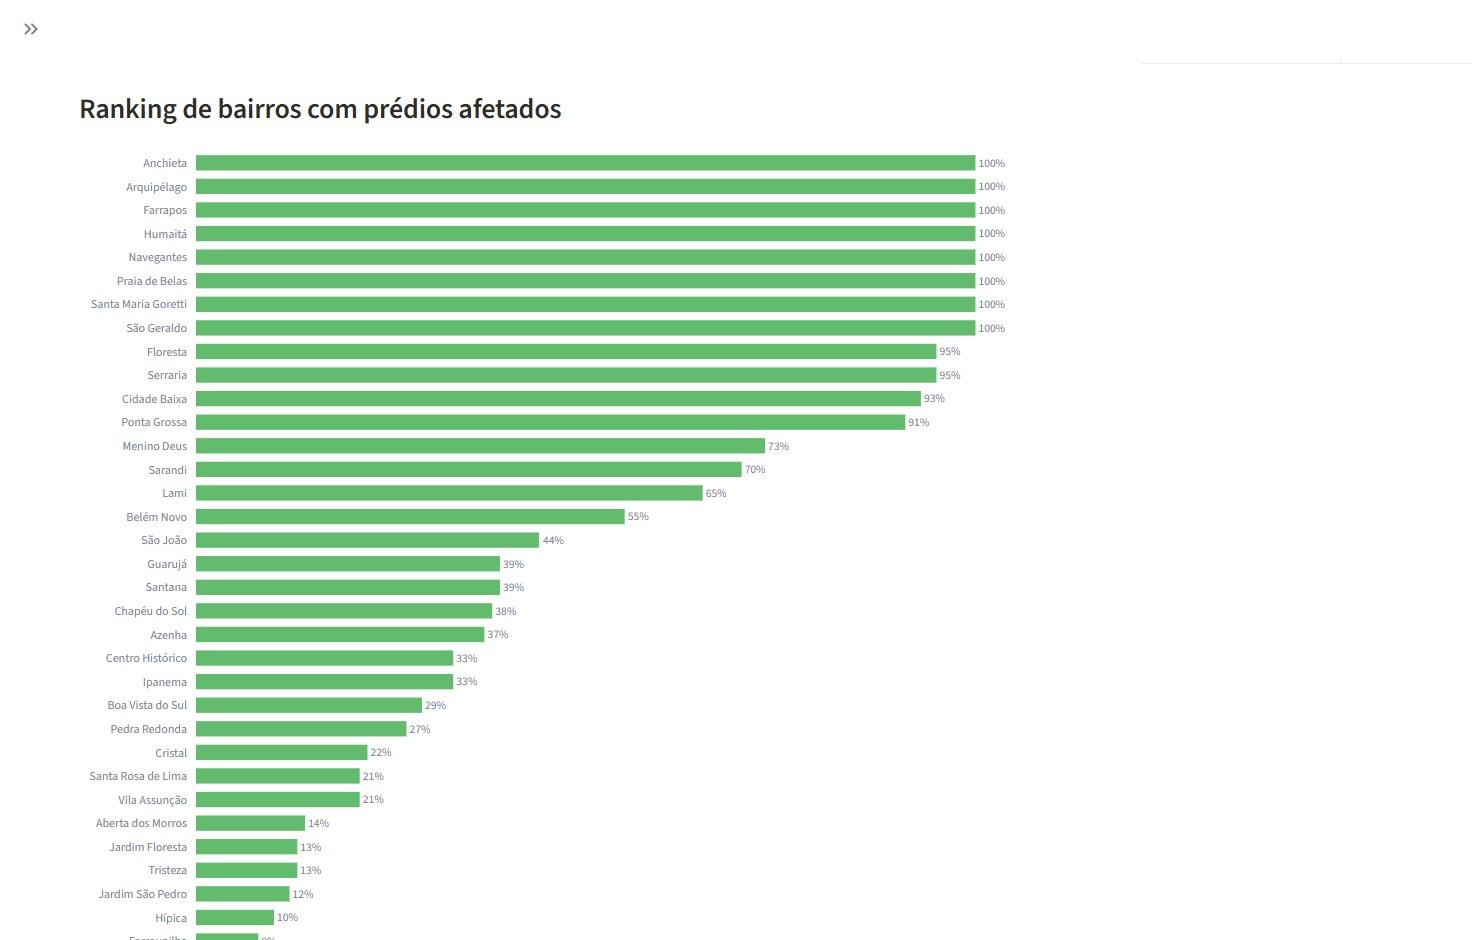
\includegraphics[width=0.75\textwidth]{assets/tela1_ranking.png}
            \caption{Ranking de bairros com prédios afetados, em porcentagem.}
            \label{fig:tela1_ranking}
        \end{figure}
        \paragrafo{Ao final da tela ficam a fonte dos dados e o aviso de limitações, como o enunciado exige. O texto exibido é: \textit{``Fonte: INCT SiMAI, simulação de inundação de Porto Alegre (arquivo data.json fornecido à turma), após limpeza pelo nosso grupo.''} e \textit{``Limitações: os números são estimativas de uma simulação, não previsões nem contagens oficiais. A população afetada supõe que os moradores se distribuem igualmente entre todos os prédios do bairro, inclusive os não residenciais. O INCT arredonda a porcentagem para cima, o que deixa a população afetada um pouco acima do cálculo exato. Corrigimos 24 valores inconsistentes da base original.''}}
        \begin{figure}[H]
            \centering
            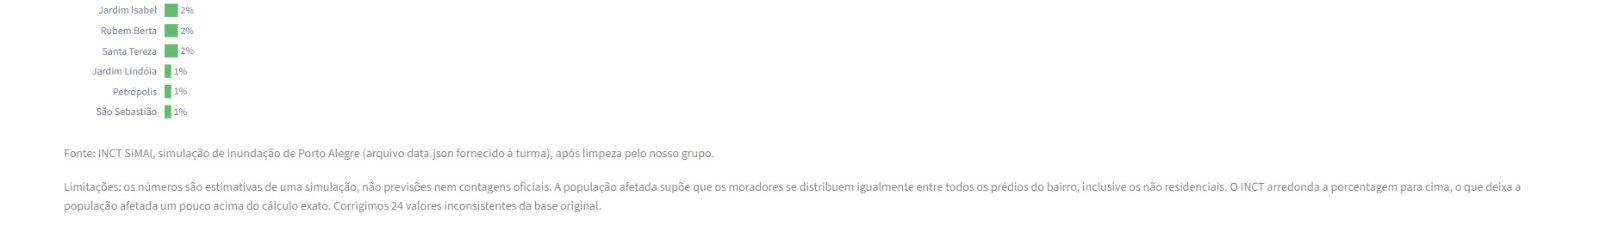
\includegraphics[width=0.9\textwidth]{assets/tela1_rodape.png}
            \caption{Final do ranking da Tela 1, com a fonte e as limitações.}
            \label{fig:tela1_rodape}
        \end{figure}

\section{Tela 2: Rotas na enchente}
    \subsection{Objetivo e como usar}
        \paragrafo{A tela mostra quais ruas ficam debaixo d'água em cada nível do Guaíba, como sair de uma área alagada e como ir de um ponto a outro só por ruas secas. O controle deslizante escolhe um dos 25 níveis das manchas de inundação, de 3,00 m a 5,30 m em passos de 0,10 m, mais o recorde de 5,35 m. Há dois modos, escolhidos em ``O que você quer ver?'':}
        \begin{itemize}
            \item \textbf{Sair da área alagada:} escolhe-se uma rua alagada (por lista ou clicando numa rua vermelha no mapa). A tela mostra a distância até a rua seca mais próxima e por qual rua se sai.
            \item \textbf{Ir de A até B sem passar pela água:} escolhem-se a partida e a chegada (por lista ou por clique no mapa, com um seletor que diz se o clique define A ou B). A tela mostra a rota por ruas secas, o desvio em relação ao caminho sem enchente e a distância sem enchente.
            \item \textbf{Mapa:} a legenda traz a área alagada (azul claro), a rua alagada (vermelho), a rua seca (verde) e a rota (azul escuro).
        \end{itemize}
    \subsection{Como funciona e por que escolhemos essas visualizações}
        \begin{itemize}
            \item \textbf{Ruas alagadas:} para cada trecho de rua, calculamos o menor nível cuja mancha de inundação o toca. Uma rua conta como alagada quando esse nível é menor ou igual ao nível escolhido. Ruas que só encostam na mancha já contam como bloqueadas.
            \item \textbf{Rotas:} as ruas viram um grafo, com o comprimento de cada trecho. A rota de A até B é o menor caminho só por ruas secas. A saída da área alagada é o menor caminho até qualquer rua seca. As distâncias são medidas pelas ruas, não em linha reta.
            \item \textbf{Mapa com camadas:} mostra de uma vez onde está a água, quais ruas servem e qual é a rota, o que um número sozinho não mostra.
            \item \textbf{Indicadores da rota:} a distância, o desvio e o caminho sem enchente mostram quanto a enchente custa a quem precisa se deslocar.
            \item \textbf{Resumo do nível:} quilômetros de ruas alagadas, parcela da malha viária, número de logradouros atingidos e maior distância até uma rua seca. Dão uma visão da cidade inteira.
        \end{itemize}
        \paragrafo{No modo de saída, a 5,35 m, quem está na rua Esp Helio Smidt precisa andar 2,0 km até a rua seca mais próxima, saindo pela Avenida Benjamin Constant.}
        \begin{figure}[H]
            \centering
            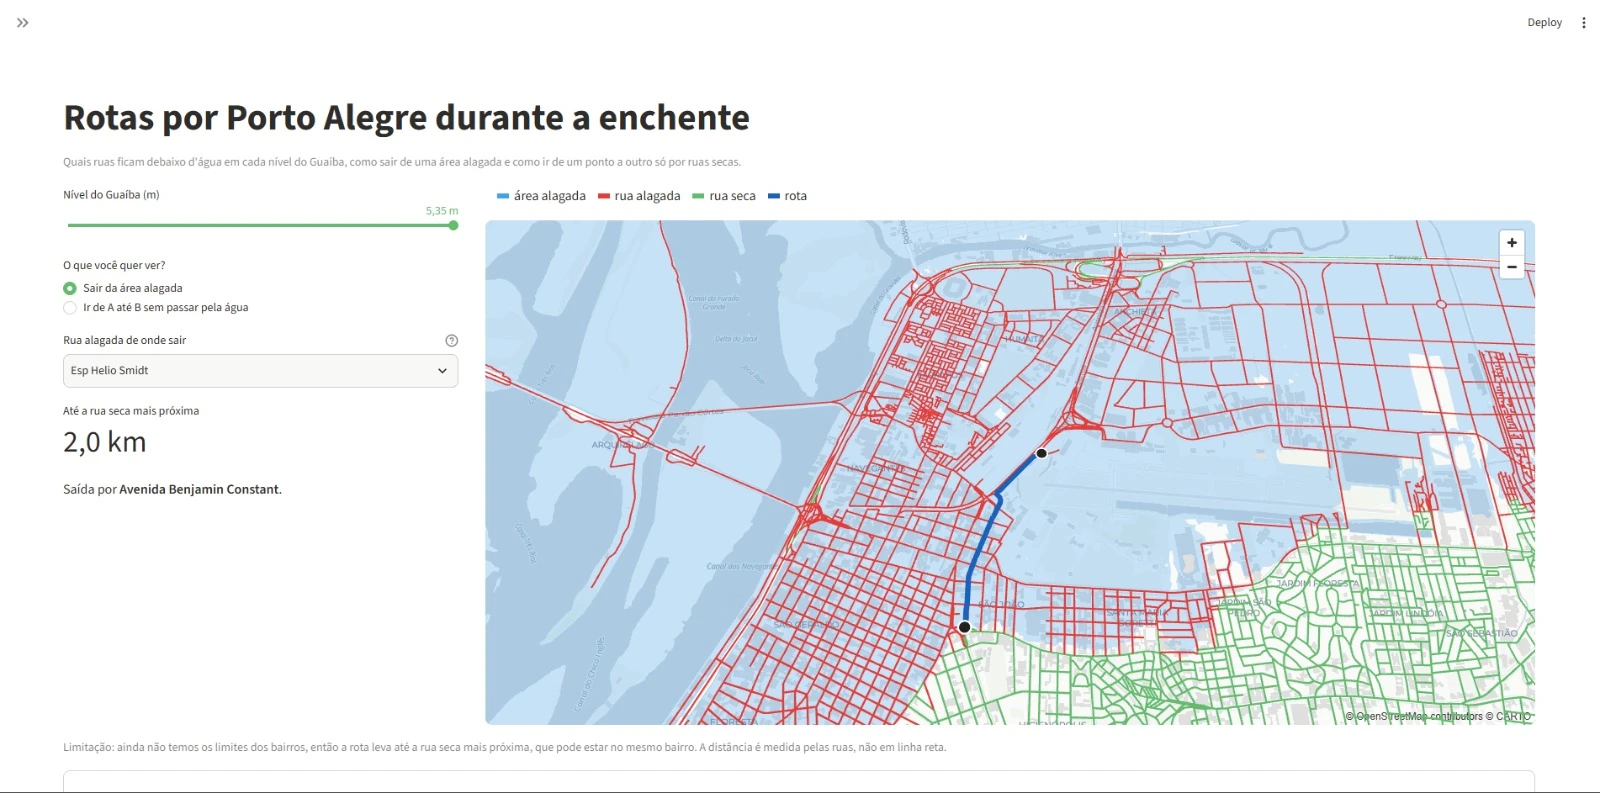
\includegraphics[width=0.9\textwidth]{assets/tela2_sair_5_35.png}
            \caption{Tela 2, modo ``Sair da área alagada'', a 5,35 m.}
            \label{fig:tela2_sair}
        \end{figure}
        \paragrafo{Outro exemplo do mesmo modo: a partir da Avenida Pátria, a saída é de 840 m, pela Rua Felicíssimo de Azevedo. Abaixo do mapa aparece o resumo do nível, com 684,1 km de ruas alagadas (21,2\% da malha viária) e 1.596 logradouros atingidos a 5,35 m. A maior distância até uma rua seca é de 12,6 km.}
        \begin{figure}[H]
            \centering
            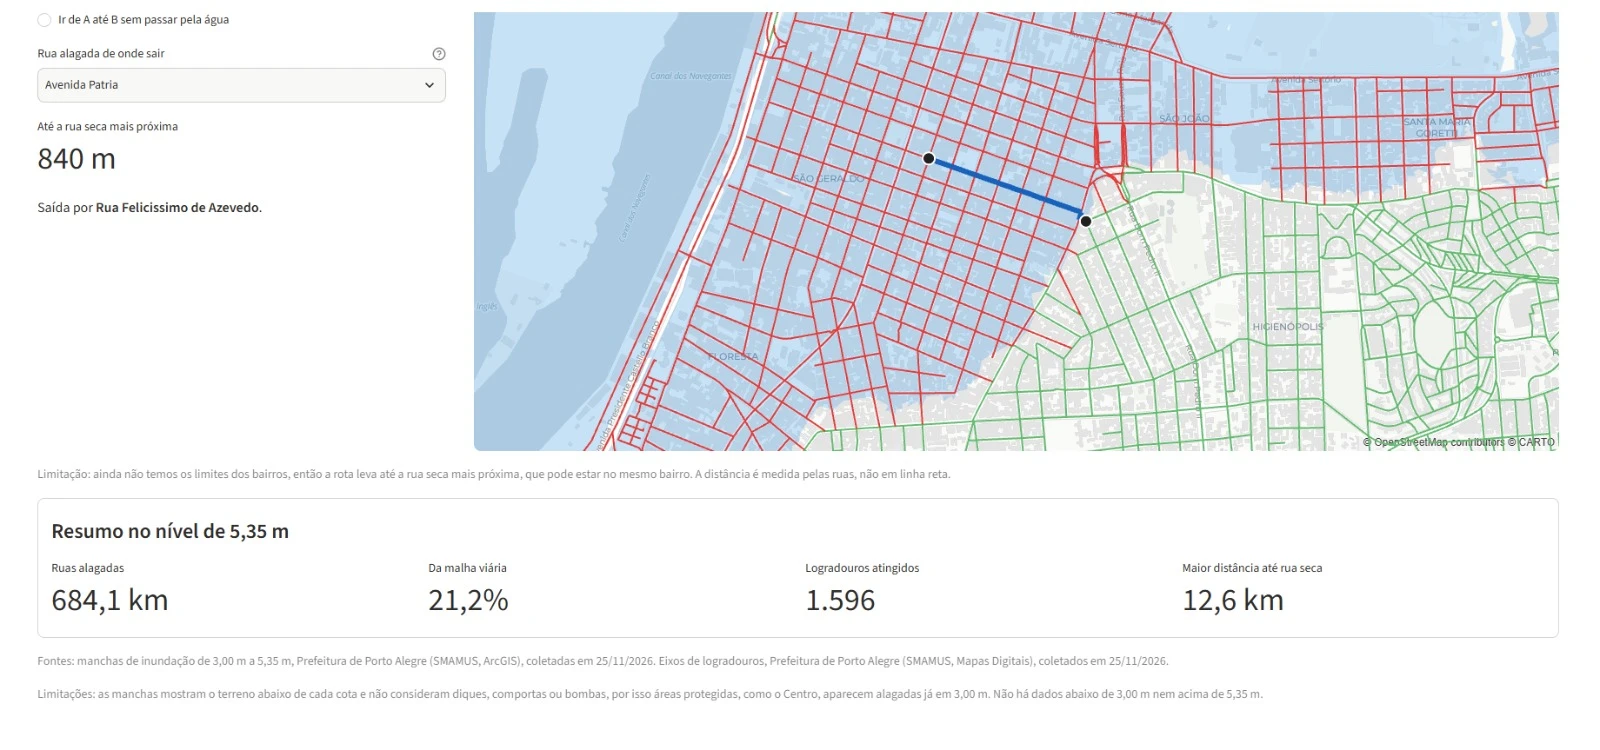
\includegraphics[width=0.9\textwidth]{assets/tela2_sair_patria.png}
            \caption{Tela 2, saída a partir da Avenida Pátria, com o resumo do nível e as fontes.}
            \label{fig:tela2_patria}
        \end{figure}
        \paragrafo{No modo de rota, a 4,20 m, ir da Rua Duque de Caxias até a Avenida Edvaldo Pereira Paiva sem passar pela água exige 15,2 km. Sem enchente seriam 2,6 km, então o desvio é de 12,6 km.}
        \begin{figure}[H]
            \centering
            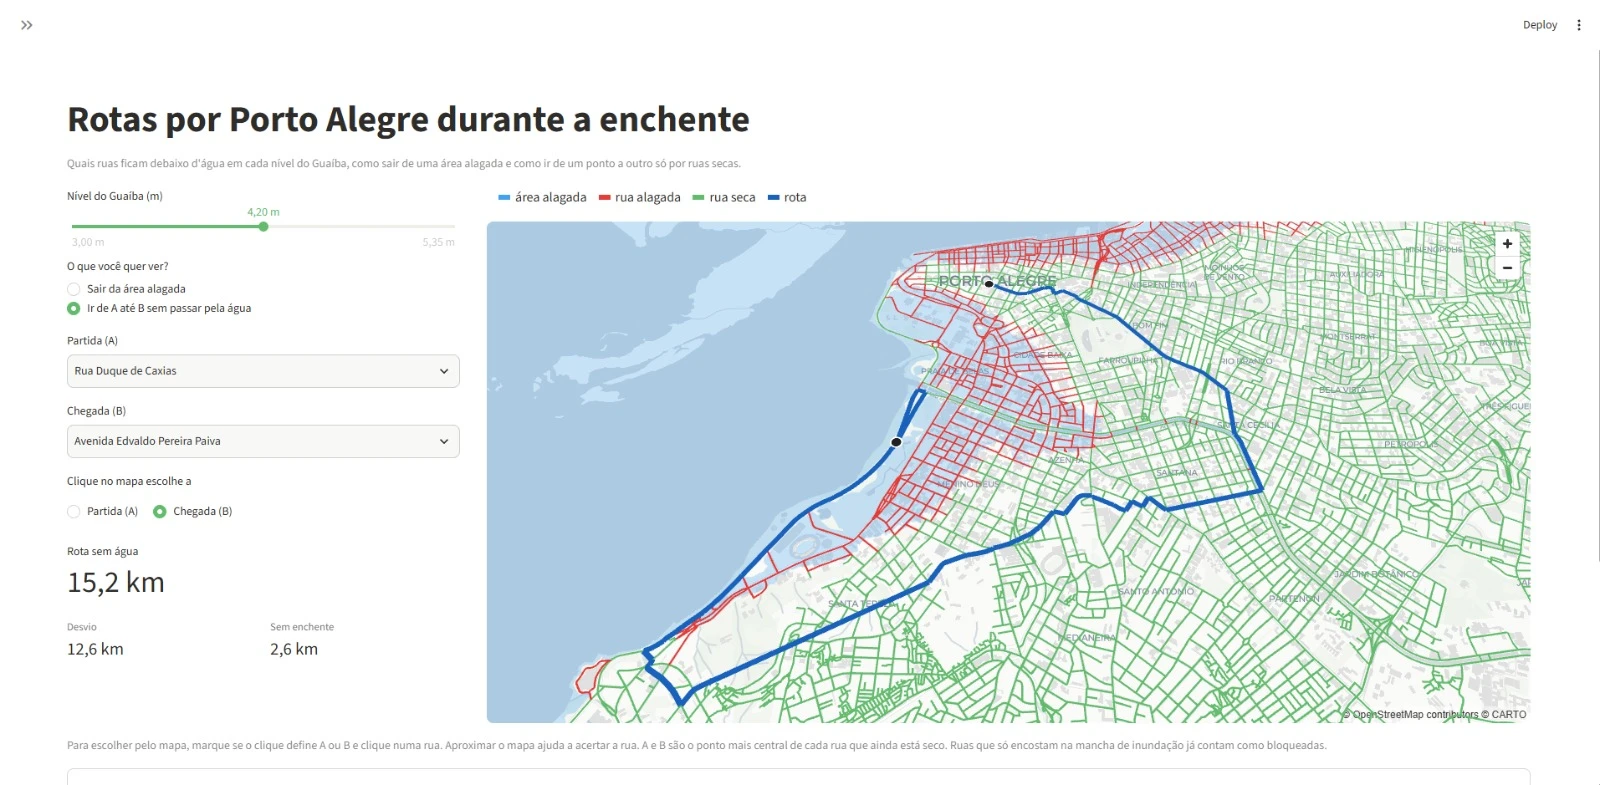
\includegraphics[width=0.9\textwidth]{assets/tela2_rota_4_20.png}
            \caption{Tela 2, modo ``Ir de A até B sem passar pela água'', a 4,20 m.}
            \label{fig:tela2_rota420}
        \end{figure}
        \paragrafo{A 5,35 m, a rota entre a Avenida Osvaldo Aranha e a Avenida Wenceslau Escobar tem 12,8 km. Sem enchente seriam 10,3 km, um desvio de 2,5 km. O mapa mostra ainda quanto da cidade fica alagado, em vermelho.}
        \begin{figure}[H]
            \centering
            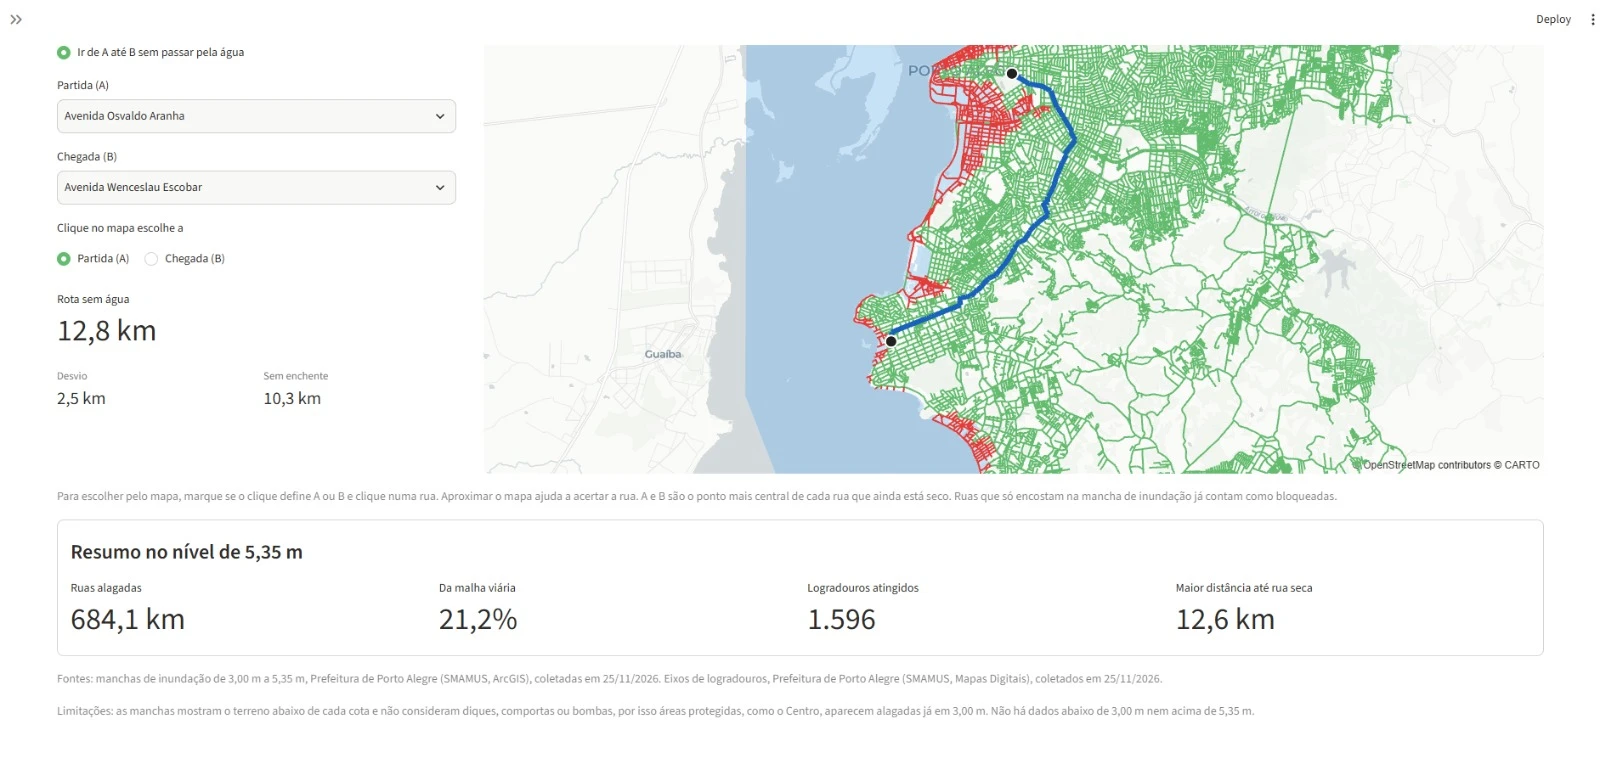
\includegraphics[width=0.9\textwidth]{assets/tela2_rota_5_35.png}
            \caption{Tela 2, rota entre duas avenidas a 5,35 m.}
            \label{fig:tela2_rota535}
        \end{figure}

\section{Como as duas telas se conectam}
    \paragrafo{O elo entre as telas é o nível do Guaíba. A Tela 1 diz quantas pessoas e quais bairros são afetados em cada nível, e a Tela 2 diz quais ruas ficam alagadas no mesmo nível. O recorde de maio de 2024 (5,35 m) aparece nas duas: como linha tracejada na curva da Tela 1 e como o nível máximo do controle da Tela 2.}
    \paragrafo{As faixas são diferentes: a simulação do INCT vai de 3,0 m a 10,0 m, e as manchas de inundação só vão de 3,00 m a 5,35 m. Ainda não ligamos as duas por bairro, porque não temos os limites dos bairros.}

\section{Limitações}
    \begin{itemize}
        \item \textbf{Estimativas:} os números da Tela 1 vêm de uma simulação, não são previsões nem contagens oficiais.
        \item \textbf{População afetada:} supõe que os moradores se distribuem igualmente entre todos os prédios do bairro, inclusive os não residenciais. Os prédios vêm do OpenStreetMap e incluem esses casos.
        \item \textbf{Arredondamento:} o INCT arredonda a porcentagem para cima, o que deixa a população afetada um pouco acima do cálculo exato (em média, 27 pessoas por linha do arquivo).
        \item \textbf{Base corrigida:} 24 valores inconsistentes foram corrigidos. Alguns valores suspeitos foram mantidos com aviso, porque só poderiam ser confirmados com a altitude do terreno.
        \item \textbf{Manchas de inundação:} mostram o terreno abaixo de cada cota e não consideram diques, comportas ou bombas. Por isso áreas protegidas, como o Centro, aparecem alagadas já em 3,00 m. A mancha também inclui o rio.
        \item \textbf{Faixa de níveis:} não há dados de manchas abaixo de 3,00 m nem acima de 5,35 m.
        \item \textbf{Ruas:} o arquivo dos eixos tem data de 2022, então ruas abertas depois podem faltar. O eixo é o centro da via e não diz a largura nem quantas faixas ficam livres. O cálculo não considera o sentido das vias nem o tempo de percurso.
        \item \textbf{Bairros na Tela 2:} sem os limites dos bairros, a rota leva até a rua seca mais próxima, que pode estar no mesmo bairro.
    \end{itemize}

\section{Atendimento aos requisitos do enunciado}
    \begin{adjustwidth}{0.3cm}{0.3cm}
    \small
    \begin{tabularx}{\linewidth}{|>{\raggedright\arraybackslash}p{5.6cm}|>{\raggedright\arraybackslash}p{2.4cm}|X|}
        \hline
        \textbf{Requisito} & \textbf{Situação} & \textbf{Onde está} \\ \hline
        \multicolumn{3}{|l|}{\textbf{Tela 1}} \\ \hline
        Controle deslizante de 3,0 m a 10,0 m, em passos de 0,1 m & Atendido & Topo da tela (Figuras \ref{fig:tela1_35} e \ref{fig:tela1_77}). \\ \hline
        Indicadores: pessoas, prédios e bairros atingidos & Atendido & Quatro indicadores no topo, com a parcela da população da cidade. \\ \hline
        Gráfico da porcentagem de prédios afetados por bairro & Atendido & Ranking de barras (Figura \ref{fig:tela1_ranking}). O mapa colorido por bairro, que era opcional, não foi feito. \\ \hline
        Curva da população afetada com o recorde de 5,35 m & Atendido & Figuras \ref{fig:tela1_35} e \ref{fig:tela1_77}. \\ \hline
        Ranking dos bairros mais afetados no nível escolhido & Atendido & Tabela dos dez bairros com mais pessoas afetadas. \\ \hline
        Aviso visível das limitações & Atendido & Rodapé (Figura \ref{fig:tela1_rodape}). \\ \hline
        \multicolumn{3}{|l|}{\textbf{Tela 2}} \\ \hline
        Base externa obtida por código & Atendido & Cotas pela API ArcGIS REST e logradouros por download automatizado do \textit{shapefile}. \\ \hline
        Pelo menos 3 visualizações e 1 filtro interativo & Atendido & Mapa de ruas e manchas, rota destacada e resumo do nível. Filtros: controle de nível, seletor de modo, seletores de rua e clique no mapa. \\ \hline
        Visualização que relacione a base externa à Tela 1 & Em parte & Relação pelo nível do Guaíba (mesmo controle e recorde de 5,35 m). Não relaciona por bairro, porque faltam os limites dos bairros. \\ \hline
        Fonte de cada dado, com link, e data de coleta & Em parte & A tela mostra a fonte e a data de coleta (Figura \ref{fig:tela2_patria}). Os links estão na seção de fontes deste relatório, e o rodapé da tela ainda não traz o link. \\ \hline
    \end{tabularx}
    \end{adjustwidth}

\section{Observações sobre a ferramenta atual do INCT}
    \paragrafo{Antes de montar o dashboard, exploramos a ferramenta atual do INCT (\url{http://vhlab.com.br/INCT/floods/}) em janela larga e no formato de celular. As observações abaixo foram o ponto de partida das nossas telas.}
    \subsection{O que funciona}
        \begin{itemize}
            \item \textbf{Resposta rápida:} no nosso teste, a página carregou em menos de 1 s e cada troca de nível respondeu em cerca de 1 s.
            \item \textbf{Análise por endereço:} mostra a mancha de inundação sobre as ruas reais e permite selecionar uma área no mapa, algo que o nosso dashboard não tem.
            \item \textbf{Histórico do nível do rio:} um gráfico dos últimos 2 a 30 dias, com o limite de 3,00 m, dá o contexto de quão perto o Guaíba está de alagar.
        \end{itemize}
    \subsection{O que atrapalha}
        \begin{itemize}
            \item \textbf{Escolha do nível pouco prática:} o nível é um campo numérico, com apenas três botões prontos (3,0 m, 5,3 m e 10,0 m) e sem controle deslizante. Na Tela 1 usamos um controle deslizante em passos de 0,1 m.
            \item \textbf{Nível não identificado nos resultados:} ao abrir, a ferramenta já mostra números (como 63.180 edificações afetadas) sem dizer a qual nível se referem. Nas nossas telas, o nível aparece junto dos resultados.
            \item \textbf{Sem comparação entre níveis nem entre bairros:} mostra só totais da cidade ou da área selecionada, sem curva do impacto nem ranking. A Tela 1 traz as duas coisas.
            \item \textbf{Pouca explicação dos números:} não encontramos como a população afetada é calculada, nem aviso de que os valores são estimativas. Nosso dashboard traz fonte e limitações no rodapé de cada tela.
        \end{itemize}

\section{Uso de IA}
    \paragrafo{Utilizamos IA (Claude) como apoio em partes do projeto. Depois de prontos, todos os arquivos foram passados para a IA para revisão, sugestões de otimização e inclusão de comentários. Os usos principais foram:}
    \begin{itemize}
        \item \textbf{Escolha das ferramentas:} decidir as bibliotecas e os formatos do projeto, principalmente por trabalharmos com dados geográficos.
        \item \textbf{Limpeza do INCT:} A lógica e as etapas da limpeza (carga, normalização, verificações, correção e saída) foram definidas por nós, e a IA ajudou a otimizar o código e sugerir outros caminhos ou verificações não vistas.
        \item \textbf{Cotas de inundação e logradouros:} exemplos de uso das bibliotecas de dados geográficos (GeoPandas e Shapely), como o reparo de geometrias, a mudança de coordenadas e o cruzamento das ruas com as manchas, e a otimização dessas operações.
        \item \textbf{Dashboards:} principalmente o layout (colunas, indicadores e legenda) e a filtragem (controle de nível, seletores de rua e clique no mapa).
        \item \textbf{Comentários e documentação:} comentários nas funções dos scripts e log de limpeza.
    \end{itemize}

\section{Reprodução e fontes}
    \paragrafo{Para reproduzir o dashboard, clone o repositório, instale as dependências com \textit{pip install -r requirements.txt} e rode \textit{python app.py}. O programa prepara os dados que ainda não existem e abre as duas telas no navegador.}
    \begin{itemize}
        \item \textbf{Cotas de inundação:} \url{https://gis-smamus.portoalegre.rs.gov.br/server/rest/services/01_PUBLICACOES/cotas_inundacao_300_535/FeatureServer/0}
        \item \textbf{Eixos de logradouros:} \url{https://prefeitura.poa.br/smamus/planejamento-urbano/mapas-digitais}
        \item \textbf{Ferramenta atual do INCT:} \url{http://vhlab.com.br/INCT/floods/}
        \item \textbf{Simulação do INCT:} arquivo \textit{data.json} fornecido à turma.
    \end{itemize}

\end{document}
